\documentclass[serif,xcolor=pdftex,dvipsnames,table,hyperref={bookmarks=false}]{beamer}

%%%%%%%%%%%%%%%%
% Change the macros below to configure the title slides
% for your course.
\newcommand{\coursename}{COMPSCI 589}
\newcommand{\instructor}{Benjamin M. Marlin}
\newcommand{\university}{University of Massachusetts Amherst}
\newcommand{\department}{College of Information and Computer Sciences}
%%%%%%%%%%%%%%%%


\newcommand{\settitlecard}[2]{
  \title[\coursename  Lecture #1] 
    {\coursename \\ Lecture #1: #2}
     \author[\instructor]{\instructor}
     \institute[\university]{
     \department\\
     \university
   }
\date{}
}

\newcommand{\maketitlepage}{
  \begin{frame}
  \titlepage
  \center{
    %If you use the slides unmodified, retain the attribution below
    \tiny{Slides by Benjamin M. Marlin (marlin@cs.umass.edu). \\
    \vspace{-1em}Created with support from National Science Foundation Award\# IIS-1350522. 
    %If you modify the slides, please retain the alternate attribution below
    %\tiny{Based on slides by Benjamin M. Marlin (marlin@cs.umass.edu). \\    
    %\vspace{-1em}Created with support from National Science Foundation Award\# IIS-1350522. 
    }                                              
  }  
  \end{frame}
}

\AtBeginSection[]
{
  \begin{frame}<beamer>{Outline}
    \tableofcontents[currentsection,subsectionstyle=hide]
  \end{frame}
}


\newcommand{\cut}[1]{}

\newcommand{\iconbox}[4]{
  \only<#1-#2>{
    \begin{columns}[T]
      \column{0.5in}
           \includegraphics[width=0.5in]{#3}
       \column{3.7in}
            #4
    \end{columns}
    \medskip
    \medskip
    \medskip
  }
}

\mode<presentation>{
  \usepackage{../beamertheme589theme}
  \setbeamercovered{invisible}
}

\mode<handout>{
  \usepackage{../beamertheme589theme}
  \setbeamercovered{transparent}
}


\usepackage[english]{babel}
\usepackage[latin1]{inputenc}
\usepackage{times}
\usepackage[T1]{fontenc}
\usepackage{amsmath}
\usepackage{amssymb}
\usepackage[noend]{algorithmic}
\usepackage{algorithm}
\usepackage{listings}

\renewcommand\mathfamilydefault{\rmdefault}

\newcommand{\setA}{\mathcal{A}}
\newcommand{\setB}{\mathcal{B}}
\newcommand{\setS}{\mathcal{S}}
\newcommand{\setV}{\mathcal{V}}
\DeclareMathOperator*{\union}{\bigcup}
\DeclareMathOperator*{\intersection}{\bigcap}
\DeclareMathOperator*{\Val}{Val}
\newcommand{\mbf}[1]{{\mathbf{#1}}}
\DeclareMathOperator*{\argmax}{arg\,max}
\DeclareMathOperator*{\argmin}{arg\,min}
\DeclareMathOperator*{\sign}{sign}
\newcommand{\deriv}[2]{\frac{\partial{#1}}{\partial{#2}}}


\settitlecard{6}{Neural Networks and Deep Learning}

\begin{document}

\maketitlepage

\section{Overview}
\subsection{Foo}

\begin{frame}[t]{Overview}

\begin{itemize}
\setlength{\itemsep}{12pt}
\item Last class we saw how basis expansion and kernels could be used to
increase the capacity of linear models in a controlled way.

\pause \item \textbf{Question:} What is the primary weakness of this approach?

\pause \item In this lecture, we'll see how artificial neural networks can learn appropriate feature representations along with decision boundaries to maximize classification accuracy.

\pause \item We'll start with the inspiration for artificial neural networks: your brain.

\end{itemize}

\end{frame}


\section{Your Brain}
\subsection{Foo}

\begin{frame}[t]{Your Brain}
\center
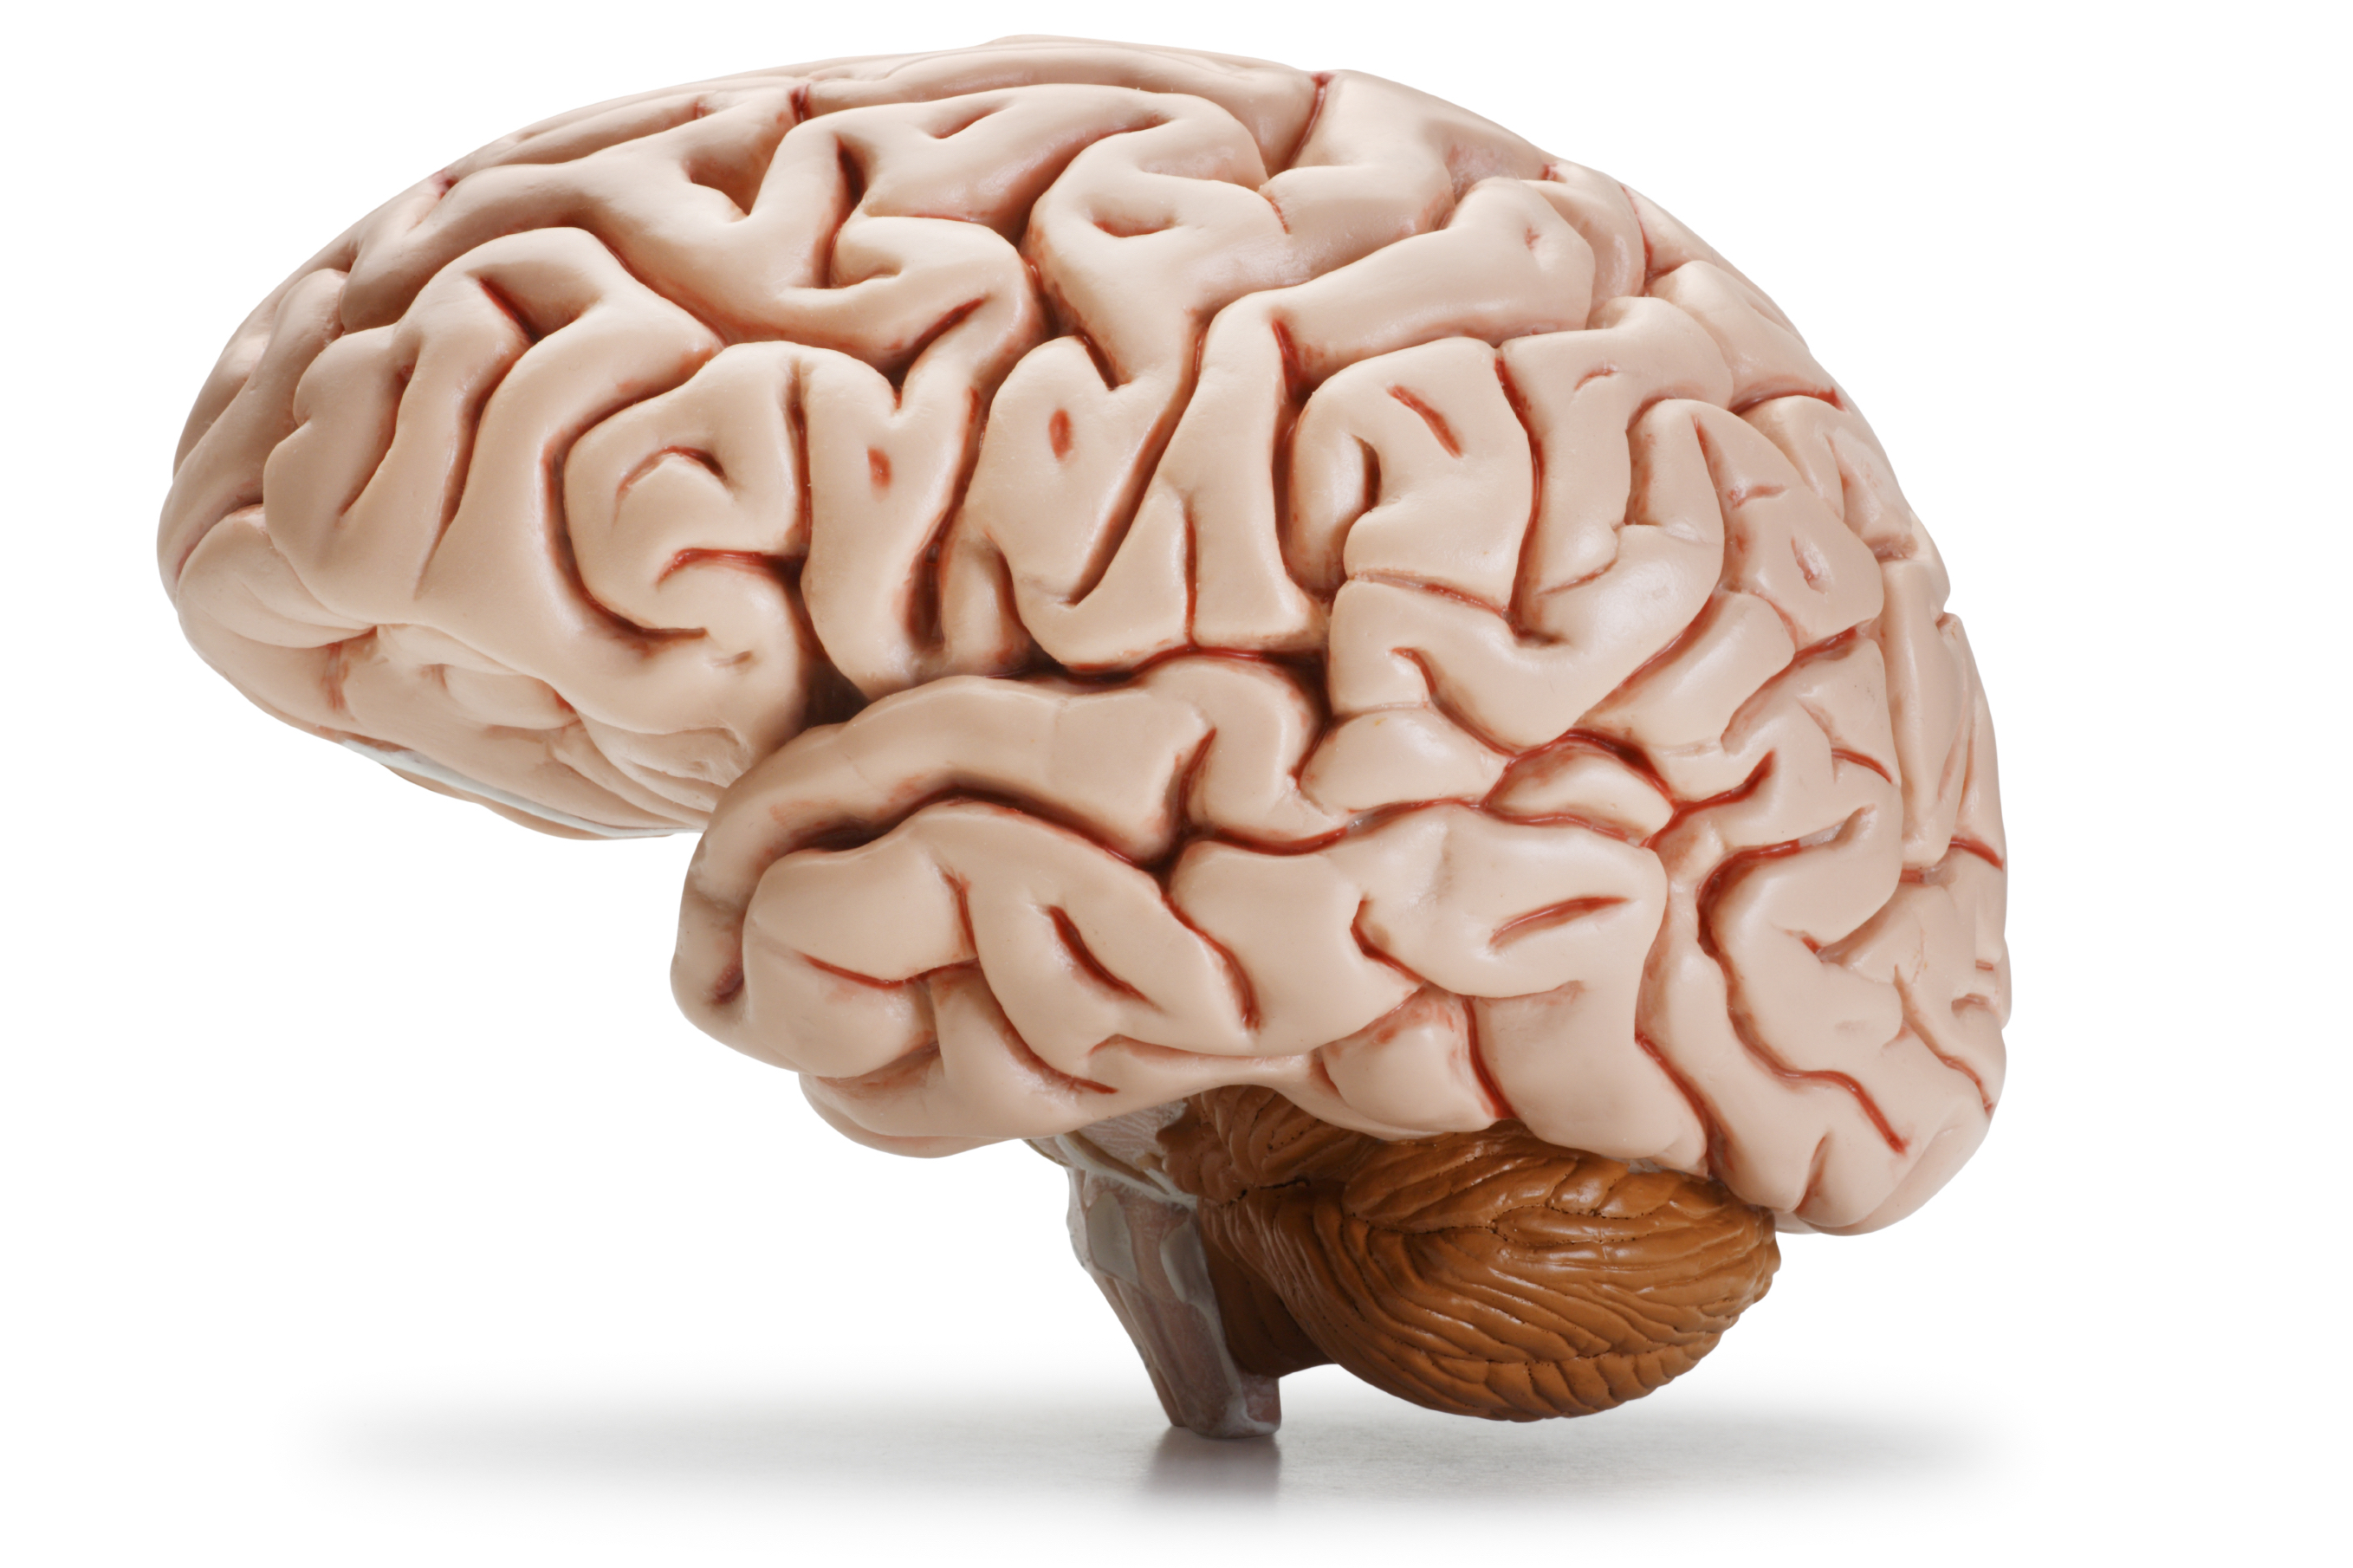
\includegraphics[width=3.8in]{../Figures/brain.jpg}
\end{frame}

\begin{frame}[t]{Brain Regions and Functions}
\center
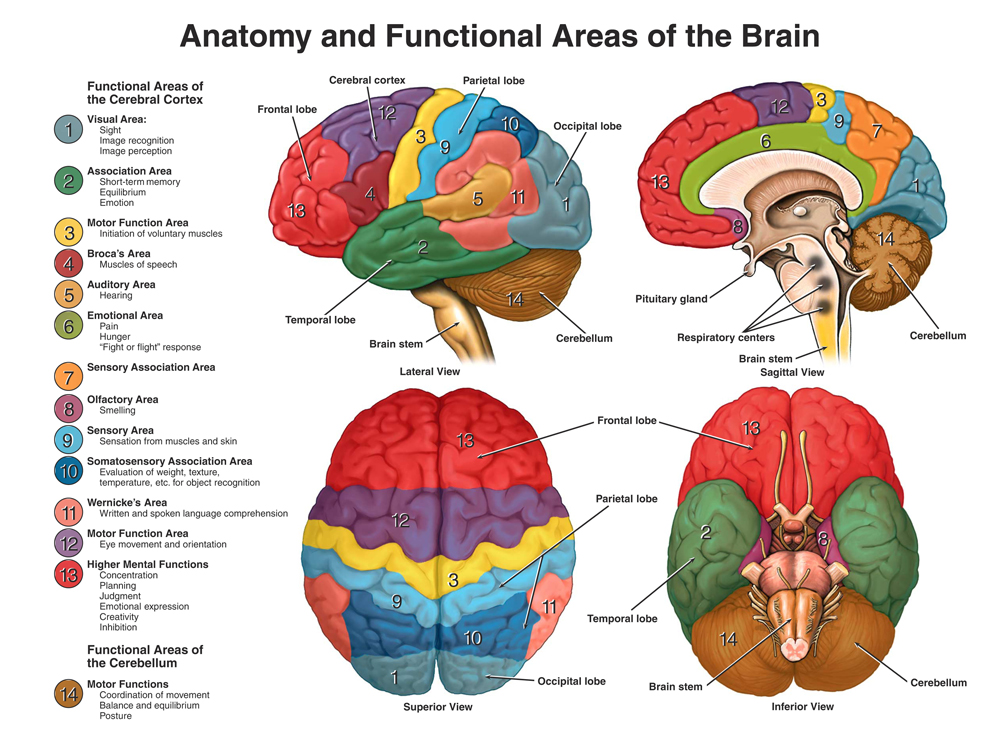
\includegraphics[width=3.8in]{../Figures/neuroanatomy.jpg}
\end{frame}

\begin{frame}[t]{Visual Areas}
\center
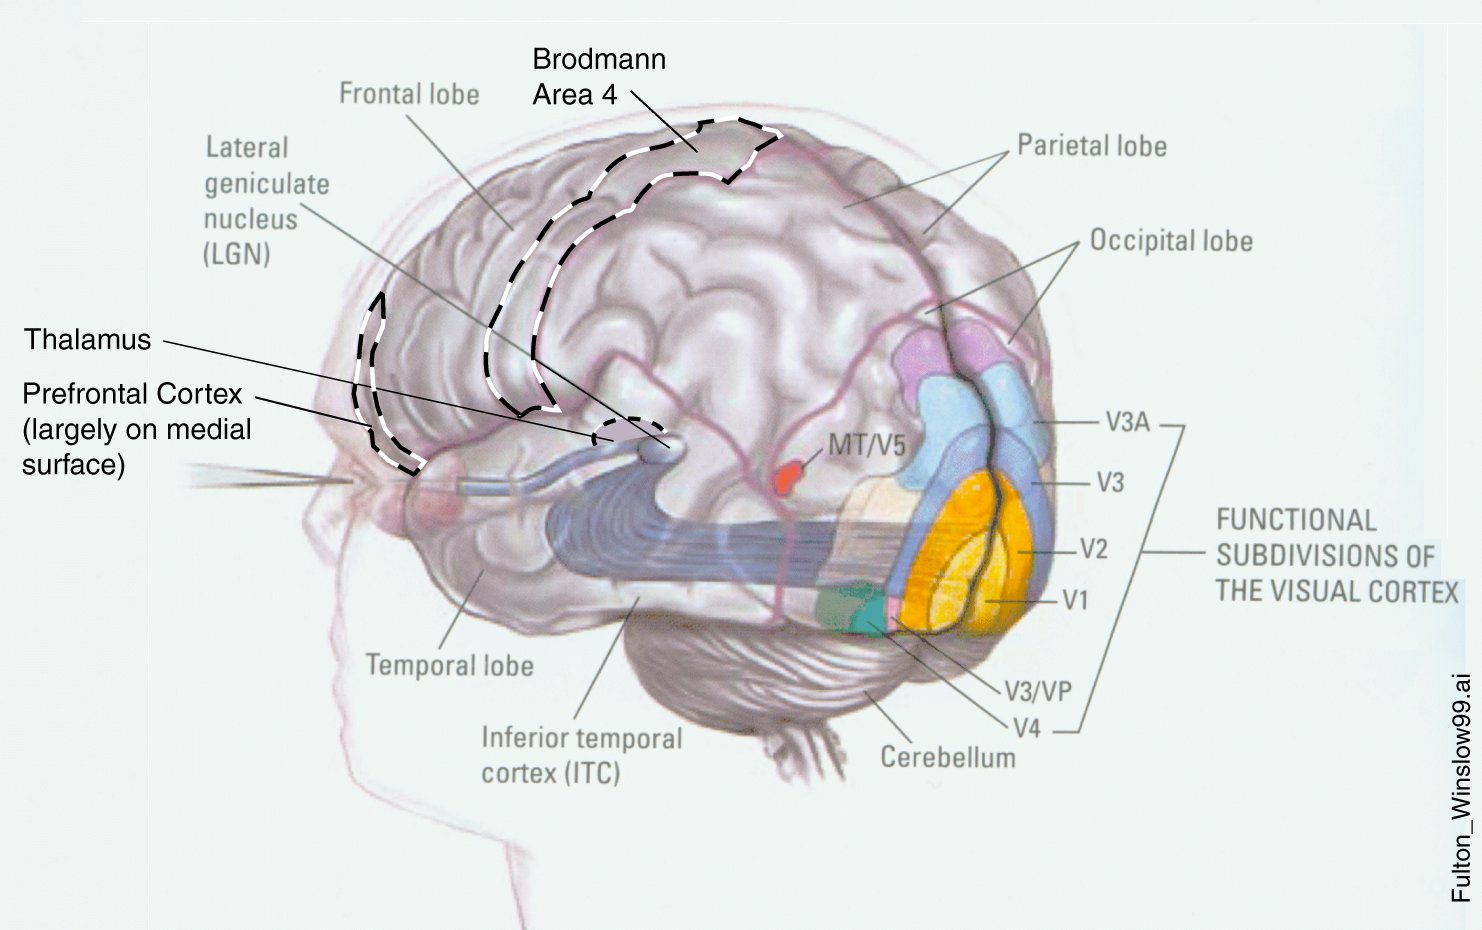
\includegraphics[width=3.9in]{../Figures/visual_areas.jpg}\\
\pause Optic nerve contains about 1 Million nerve fibers.
\end{frame}

\begin{frame}[t]{Cortical Columns}
\center
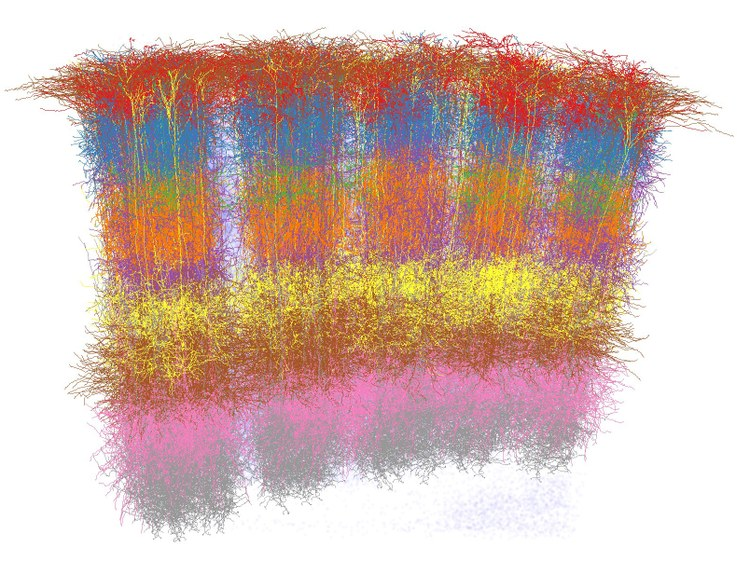
\includegraphics[width=3.5in]{../Figures/cortical_columns.jpg}
\end{frame}

\begin{frame}[t]{Neurons}
\center
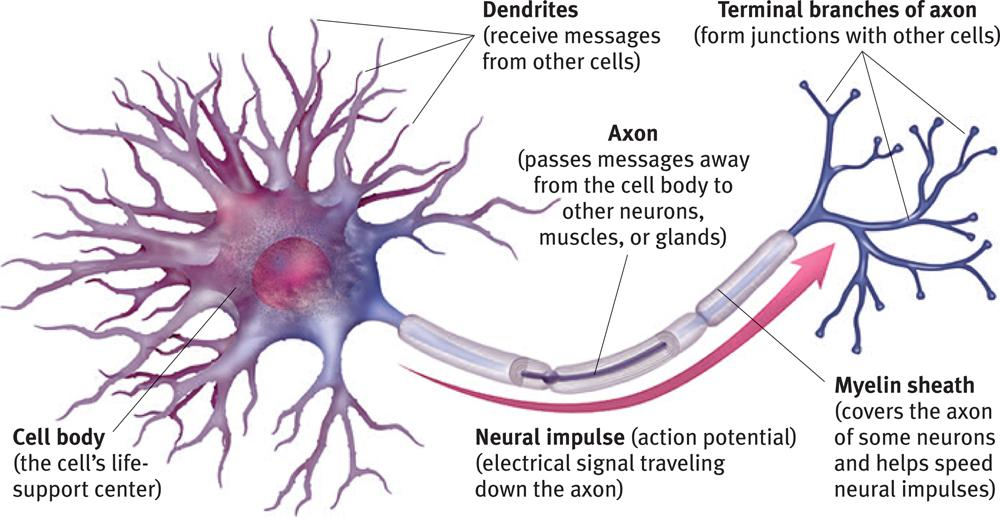
\includegraphics[width=4in]{../Figures/neuron.jpg}\\
\pause Your brain contains about 100 Billions neurons. 
\end{frame}

\begin{frame}[t]{Visual Receptive Fields}
\center
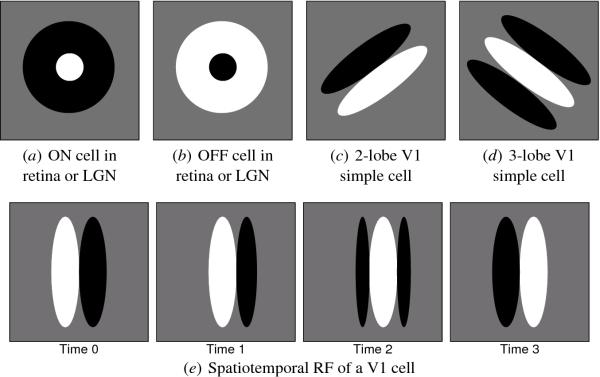
\includegraphics[width=4in]{../Figures/receptive_fields.jpg}\\ 
\end{frame}

\begin{frame}[t]{Mapping Receptive Fields in Live Subjects}
\center
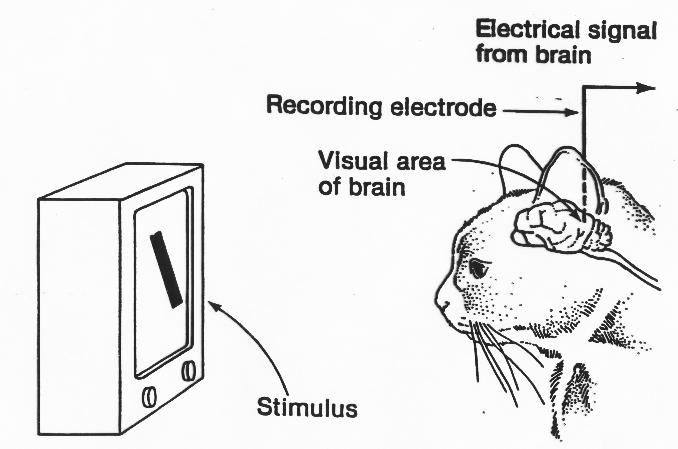
\includegraphics[width=3.5in]{../Figures/cat_experiment.jpg}\\ 
Hubel and Wiesel earned the Nobel Prize in Physiology or Medicine in 1981 for this work.\\
\end{frame}



\section{Neural Networks}
\subsection{Foo}

\begin{frame}[t]{McCulloch and Pitts Neuron (1943)}
\center
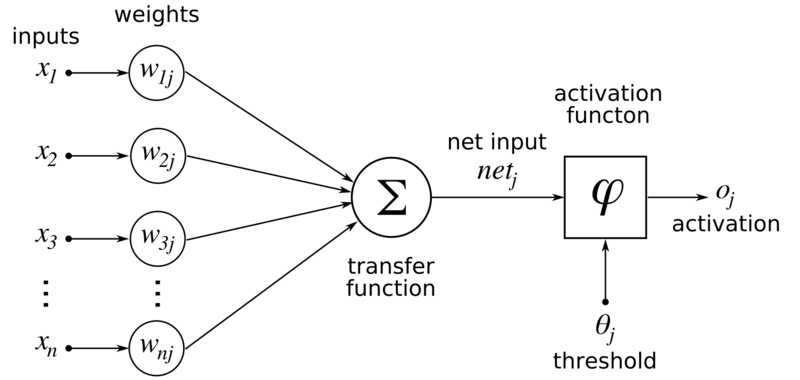
\includegraphics[width=4in]{../Figures/pitts_neuron.png}\\
\pause Assuming $\varphi() = \sign()$, what model is this?
\end{frame}

\begin{frame}[t]{The Perceptron (1950)}

The Perceptron is a simple online algorithm for adapting the weights in a
McCulloch/Pitts neuron. It was developed in the 1950s by Rosenblatt at Cornell.

\center
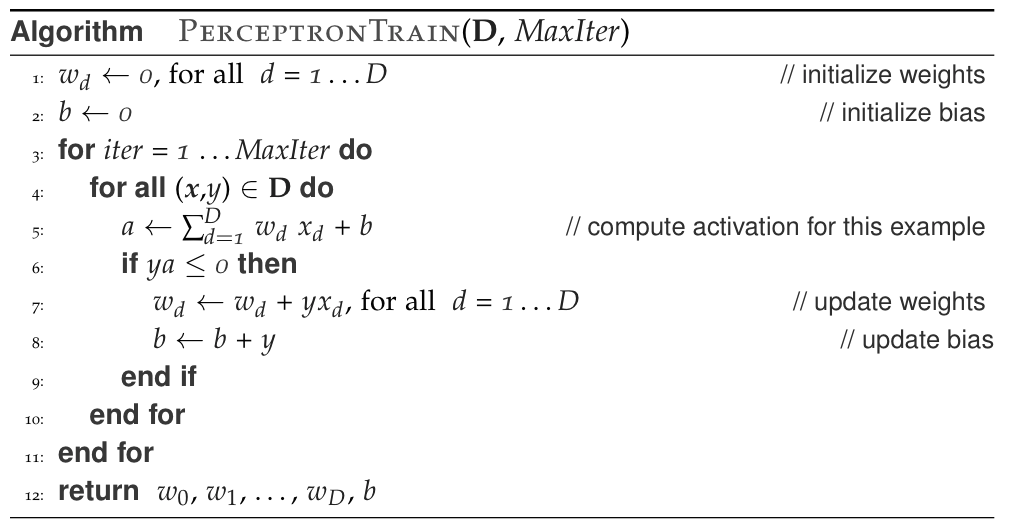
\includegraphics[width=4in]{../Figures/perceptron_algorithm.png}

\end{frame}

\begin{frame}[t]{Limitations of Single Layer Perceptrons}

\begin{itemize}
\setlength{\itemsep}{8pt}

\item The representational limitations of the single-layer perceptron were not well understood at first in the AI community.

\pause\item In 1969, Minsky and Papert at MIT popularized a set of arguments showing that the single-layer perceptron could not learn certain classes of functions (including XOR). 

\pause\item They also showed that more complex functions could be represented using a
\textit{multi-layer perceptron} or MLP, but no one knew how to learn them from examples.

\pause\item This led to a shift away from mathematical/statistical models in AI toward
logical/symbolic models.

\end{itemize}

\end{frame}


\begin{frame}[t]{Multi-Layer Perceptron}

\center
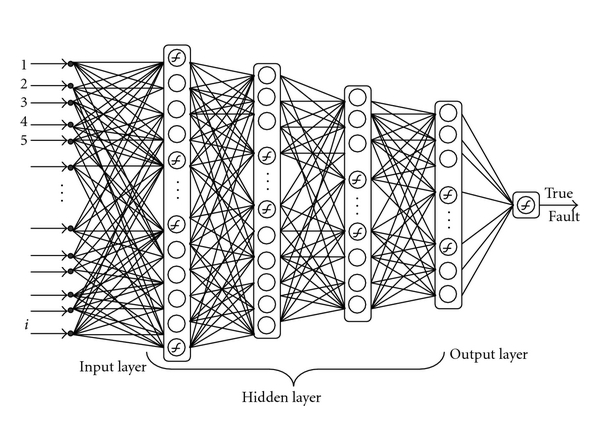
\includegraphics[width=4in]{../Figures/sigmoid_network.jpg}

\end{frame}


\begin{frame}[t]{Sigmoid Neural Networks}
The solution to MLP learning turned out to be: 
\begin{enumerate}
\setlength{\itemsep}{8pt}

\item Make the hidden layer non-linearities smooth (sigmoid/logistic) functions:

\begin{align}
h^{(1)}_k &= \frac{1}{1+\exp(-(\sum_{d}w_{dk}x_d + b_{dk}))}\\
h^{(i)}_k &= \frac{1}{1+\exp(-(\sum_{l}w_{lk}h^{(i-1)}_l + b_{lk}))}
\end{align}

\pause \item Make the output layer non-linearity a smooth (sigmoid/logistic/softmax) function.

\pause \item Use standard numerical optimization methods (gradient descent) to learn the parameters. The algorithm is known as Backpropagation and was popularized by Rumelhart, Hinton and Williams in the 1980s.  
\end{enumerate}

\end{frame}

\begin{frame}[t]{Sigmoid Neural Network Properties} 
\begin{itemize}
\setlength{\itemsep}{8pt}

\item It can be shown that a sigmoid network with one hidden layer (of unbounded size) is a universal function approximator. 

\pause\item In terms of classification, this means neural networks with one hidden layer (of unbounded size) can represent any decision boundary and thus have infinite capacity.

\pause\item It was also shown that deep networks can be exponentially more efficient at representing certain types of functions than shallow networks.

\pause\item Demo!

\end{itemize}

\end{frame}


\begin{frame}[t]{More Failures}
\begin{itemize}
\setlength{\itemsep}{8pt}

\item Through the 1990s is became clear that while these models could represent arbitrarily complex functions and that deep networks should work better than shallow networks, no one could effectively train deep networks.

\pause\item This led to a shift away from neural networks towards probabilistic/statistical  models and SVMs through the late 1990s and 2000s. 

\pause\item Only a few groups continued to work on neural network models during this time period (Hinton, LeCun, Bengio, Ng).

\end{itemize}
\end{frame}

\section{Deep Learning}
\subsection{foo}

\begin{frame}[t]{Deep Learning}
The solution to the deep learning problem (as of right now) appears to be:

\begin{enumerate}
\setlength{\itemsep}{8pt}

\item Have access to lots of labeled data (ie: millions of examples).

\pause\item Make the non-linearities non-smooth again (rectified linear units, ReLU):

\begin{align}
h^{(1)}_k &= \max(0,\sum_{d}w_{dk}x_d + b_{dk}))\\
h^{(i)}_k &= \max(0,\sum_{l}w_{lk}h^{(i-1)}_l + b_{lk}))
\end{align}

\end{enumerate}
\end{frame}


\begin{frame}[t]{Deep Learning}
The solution to the deep learning problem (as of right now) appears to be:

\begin{enumerate}
\setlength{\itemsep}{8pt}

\item Have access to lots of labeled data (ie: millions of examples).

\pause\item Make the non-linearities non-smooth again (rectified linear units, ReLU):

\begin{align}
h^{(1)}_k &= \max(0,\sum_{d}w_{dk}x_d + b_{dk}))\\
h^{(i)}_k &= \max(0,\sum_{l}w_{lk}h^{(i-1)}_l + b_{lk}))
\end{align}

\end{enumerate}
\end{frame}

\begin{frame}[t]{Deep Learning}
The solution to the deep learning problem (as of right now) appears to be:

\begin{enumerate}
\setlength{\itemsep}{8pt}
\setcounter{enumi}{2}
\item Use somewhat improved optimization methods for non-smooth functions (accelerated stochastic sub-gradient descent) to learn the parameters.

\pause\item Use new regularization schemes based on randomly zeroing-out nodes in the
network.

\pause\item Do the computing on a GPU with 1000s of cores and 10s of GB of RAM for a massive 20-30X speedup (go SIMD!). Model training takes 10 days for large vision problems instead of 1 year.

\end{enumerate}
\end{frame}

\begin{frame}[t]{Deep Learning Applications}

\begin{itemize}
\setlength{\itemsep}{8pt}

\item Deep learning models using these basic ingredients have become dominant in AI over the last few years starting with computer vision and moving on to other areas including speech recognition.

\pause\item Many companies use deep learning-based vision systems to analyze photos and images.

\pause\item Google and others switched to deep-learning based speech recognition systems after it was shown to lead to substantial reductions in the word error rate.
\end{itemize}
\end{frame}

\begin{frame}[t]{Deep Learning For Vision}

Deep learning for vision uses a modified deep architecture called a \textit{convolutional network} or convnet that learns small patches of weights (or filters)
and replicates (convolves) them over an image. 

{\center
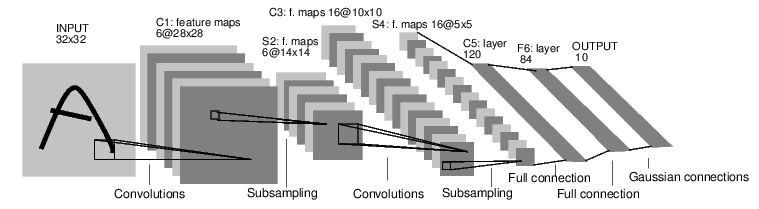
\includegraphics[width=4in]{../Figures/convnet.png}
\vspace{1em}
}

\pause This architecture is also from the 1980s and was 
directly inspired by the structure of the visual areas of the brain.

\end{frame}


\begin{frame}[t]{Learned Receptive Fields}

\center
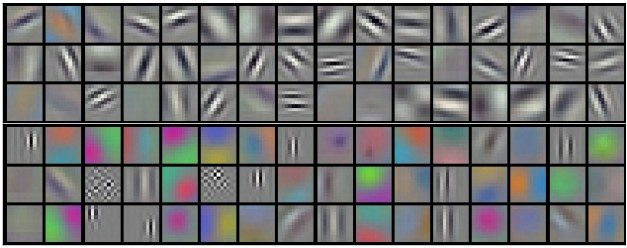
\includegraphics[width=4in]{../Figures/nn_filters.jpg}

\end{frame}

\begin{frame}[t]{Learned Receptive Fields}

\center
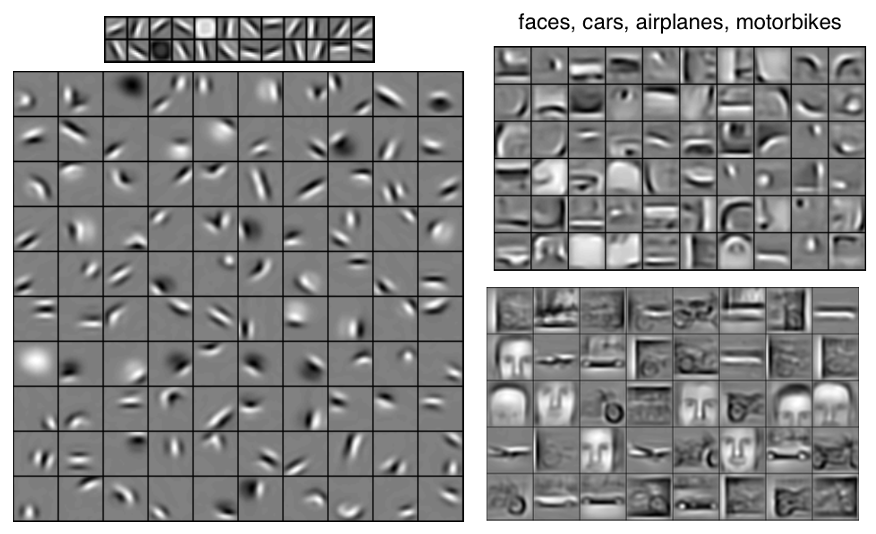
\includegraphics[width=4in]{../Figures/rbm_filters.png}

\end{frame}

\begin{frame}[t]{Deep Learning Demos}

\begin{itemize}
\setlength{\itemsep}{8pt}

\item Digit Recognition: \url{http://cs.stanford.edu/people/karpathy/convnetjs/demo/mnist.html}

\item Image Classification: \url{http://www.clarifai.com/\#demo}

\item Image Classification: \url{http://deeplearning.cs.toronto.edu/}

\item Image Description: \url{http://deeplearning.cs.toronto.edu/i2t}

\item Handwriting Generation: \url{http://www.cs.toronto.edu/\~graves/handwriting.cgi}

\end{itemize}

\end{frame}




\end{document}
